\documentclass[usepdftitlre=false, debug]{beamer}

\usepackage[francais]{babel}
\usepackage[T1]{fontenc}
\usepackage[ansinew]{inputenc}
\usepackage{lmodern}
\usepackage{graphicx}
\usepackage{listings}
\usepackage{color}
\usepackage{pgf}
\usepackage{tikz}
\usetikzlibrary{arrows,automata}



%%%%%%%%%%%%%%%%%%%%%%%%%%%%%%%%%%%%%%%%%%%%%%%%%%%%%%%%%%%%%%%%%%%%%%%%%%%%%%%%%%%%%%%%%%%%%%%%
\usetheme{Rochester}
\usecolortheme{default}

\title{WinEchek}
\author{Mathis Deloge, Antoine Petot, Ange Picard, Arthur Carchi, Lucas Fougerouse, Vincent Dereclenne}
\institute{IUT Informatique Dijon / Auxerre}
\date{Lundi 14 Novembre 2016}
%%%%%%%%%%%%%%%%%%%%%%%%%%%%%%%%%%%%%%%%%%%%%%%%%%%%%%%%%%%%%%%%%%%%%%%%%%%%%%%%%%%%%%%%%%%%%%%%



\definecolor{mygreen}{rgb}{0,0.6,0}
\definecolor{mygray}{rgb}{0.5,0.5,0.5}
\definecolor{mymauve}{rgb}{1,0,0}

\lstset{ %
  backgroundcolor=\color{gray!30!white},   % choose the background color
  basicstyle=\small\ttfamily,        % size of fonts used for the code
  breaklines=true,                 % automatic line breaking only at whitespace
  captionpos=b,                    % sets the caption-position to bottom
  commentstyle=\color{mygreen},    % comment style
  escapeinside={\%*}{*)},          % if you want to add LaTeX within your code
  keywordstyle=\color{blue},       % keyword style
  stringstyle=\color{mymauve},     % string literal style
	numbers=left,
	frame=leftline,
	xleftmargin=42pt
}

\setbeamertemplate{navigation symbols}{%
\insertbackfindforwardnavigationsymbol
}

\setbeamercolor{background canvas}{bg=yellow!10!white}

\AtBeginSection[]
{
  \begin{frame}
  \frametitle{Sommaire}
  \tableofcontents[currentsection, hideothersubsections]
  \end{frame}
}

\begin{document}

\begin{frame}
	\titlepage
\end{frame}

\section{Fonctionnalit�s}
\subsection{Menu}
\begin{frame}
	\frametitle{Menu}
	\begin{block}{Un menu principal}
		\begin{itemize}
			\item Jouer en local : Pour jouer une partie locale contre un autre joueur
			\item Jouer en r�seau : Pour jouer une partie en r�seau
			\item Jouer contre l'ordinateur : Pour jouer une partie contre un ordinateur
			\item Param�tres : Permet d'acc�der aux param�tres de WinEchek
			\item Contribuer : Pour participer au d�veloppement de WinEchek
		\end{itemize}
	\end{block}
	\begin{center}
	 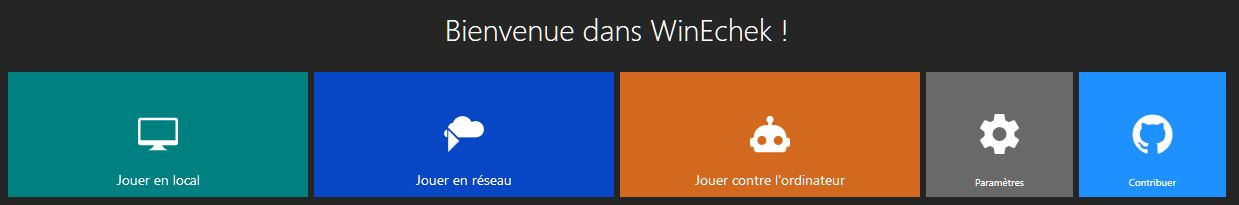
\includegraphics[width=10cm]{Images/MenuPrincipal.jpg}
	\end{center}
\end{frame}

\subsubsection{Jouer en local}
\begin{frame}
	\frametitle{Jouer en local}
	\begin{block}{Un sous menu}
		\begin{itemize}
		 \item Cr�er une nouvelle partie
		 \item Reprendre une partie
		\end{itemize}
	\end{block}
	\begin{center}
	 
\includegraphics[width=9cm]{Images/JouerEnLocal.jpg}
	\end{center}
\end{frame}


\subsection{Interface graphique}
\begin{frame}
	\frametitle{Interface graphique}
	\begin{block}{GUI}
		\begin{itemize}
		 \item Application responsive
		 \item Affichage d'un plateau de jeu
		 \item Affichage de pi�ce sur le plateau de jeu
		 \item D�placement des pi�ces sur le plateau
		 \item Diff�rentes options de partie
		\end{itemize}
	\end{block}
\end{frame}

\subsubsection{Application responsive}
\begin{frame}
	\frametitle{Une application enti�rement responsive}
	\begin{center}
	 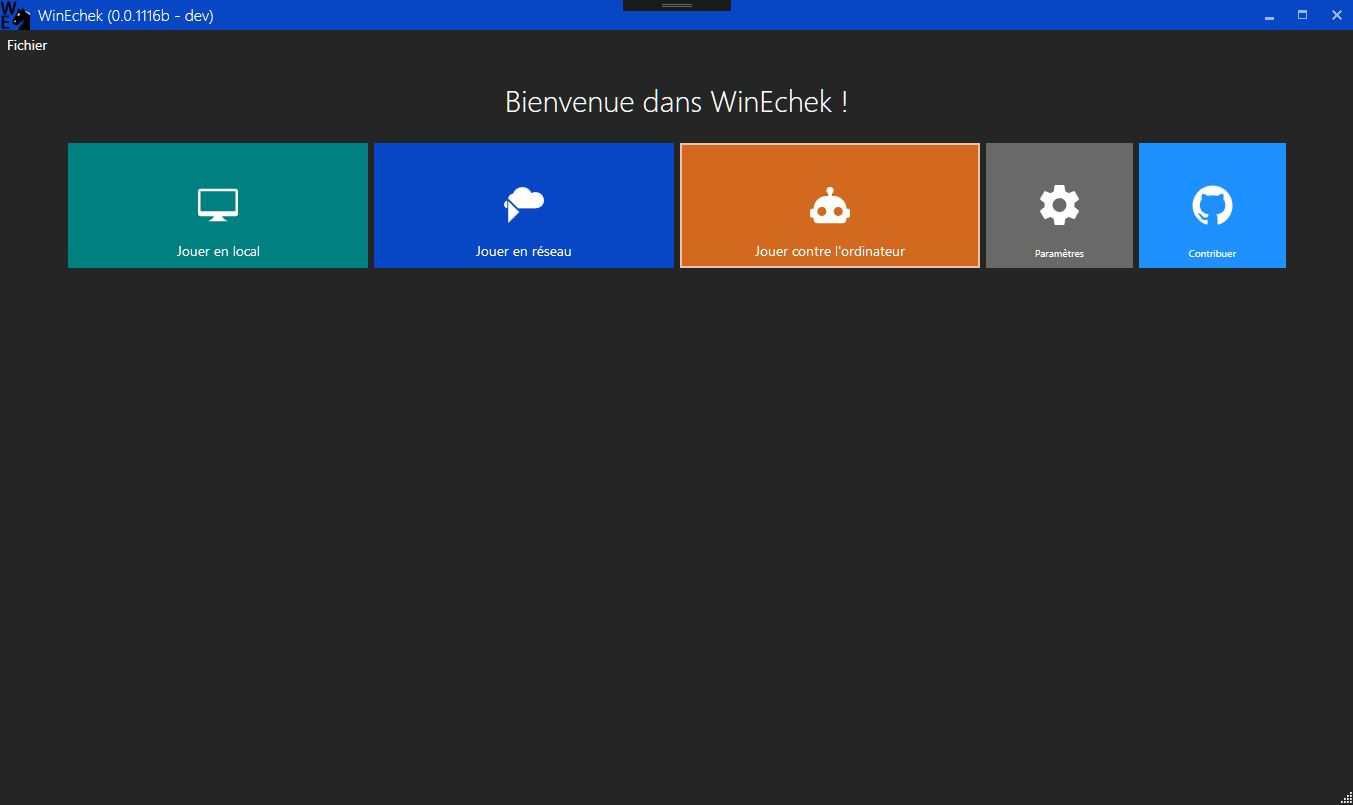
\includegraphics[width=10cm]{Images/responsive1.jpg}
	\end{center}
\end{frame}

\begin{frame}
	\frametitle{Une application enti�rement responsive}
	\begin{center}
	 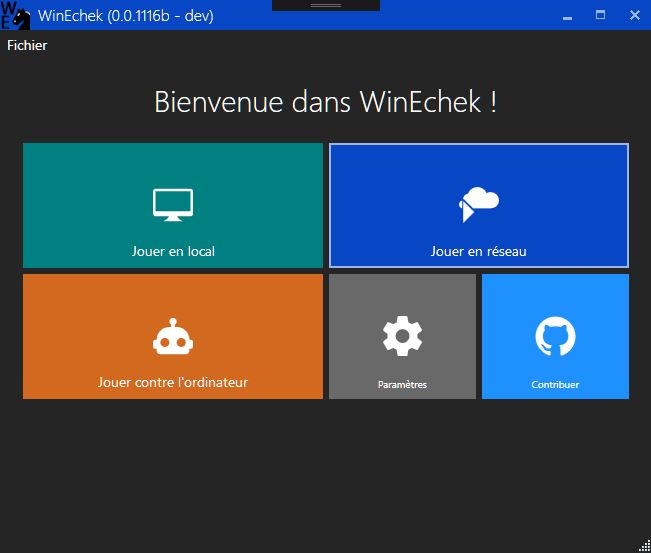
\includegraphics[width=8cm]{Images/responsive3.jpg}
	\end{center}
\end{frame}

\begin{frame}
	\frametitle{Une application enti�rement responsive}
	\begin{center}
	 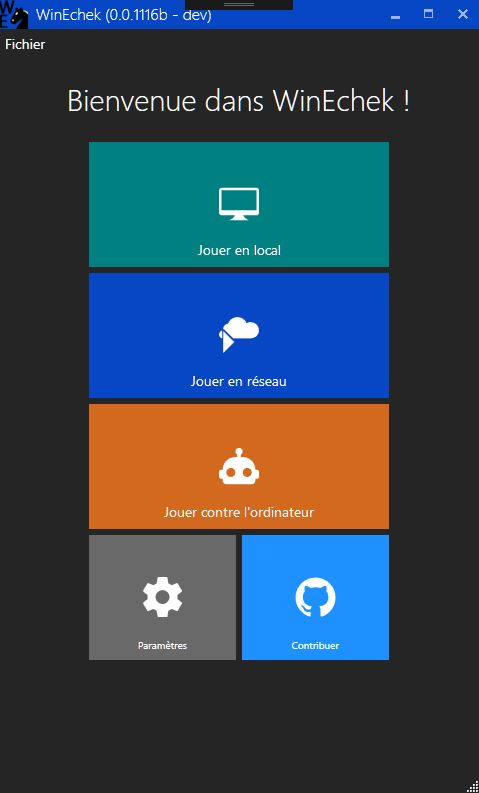
\includegraphics[width=4cm]{Images/responsive2.jpg}
	\end{center}
\end{frame}

\subsubsection{Affichage du plateau et des pi�ces}
\begin{frame}
	\frametitle{Affichage du plateau et des pi�ces}
	\begin{center}
	 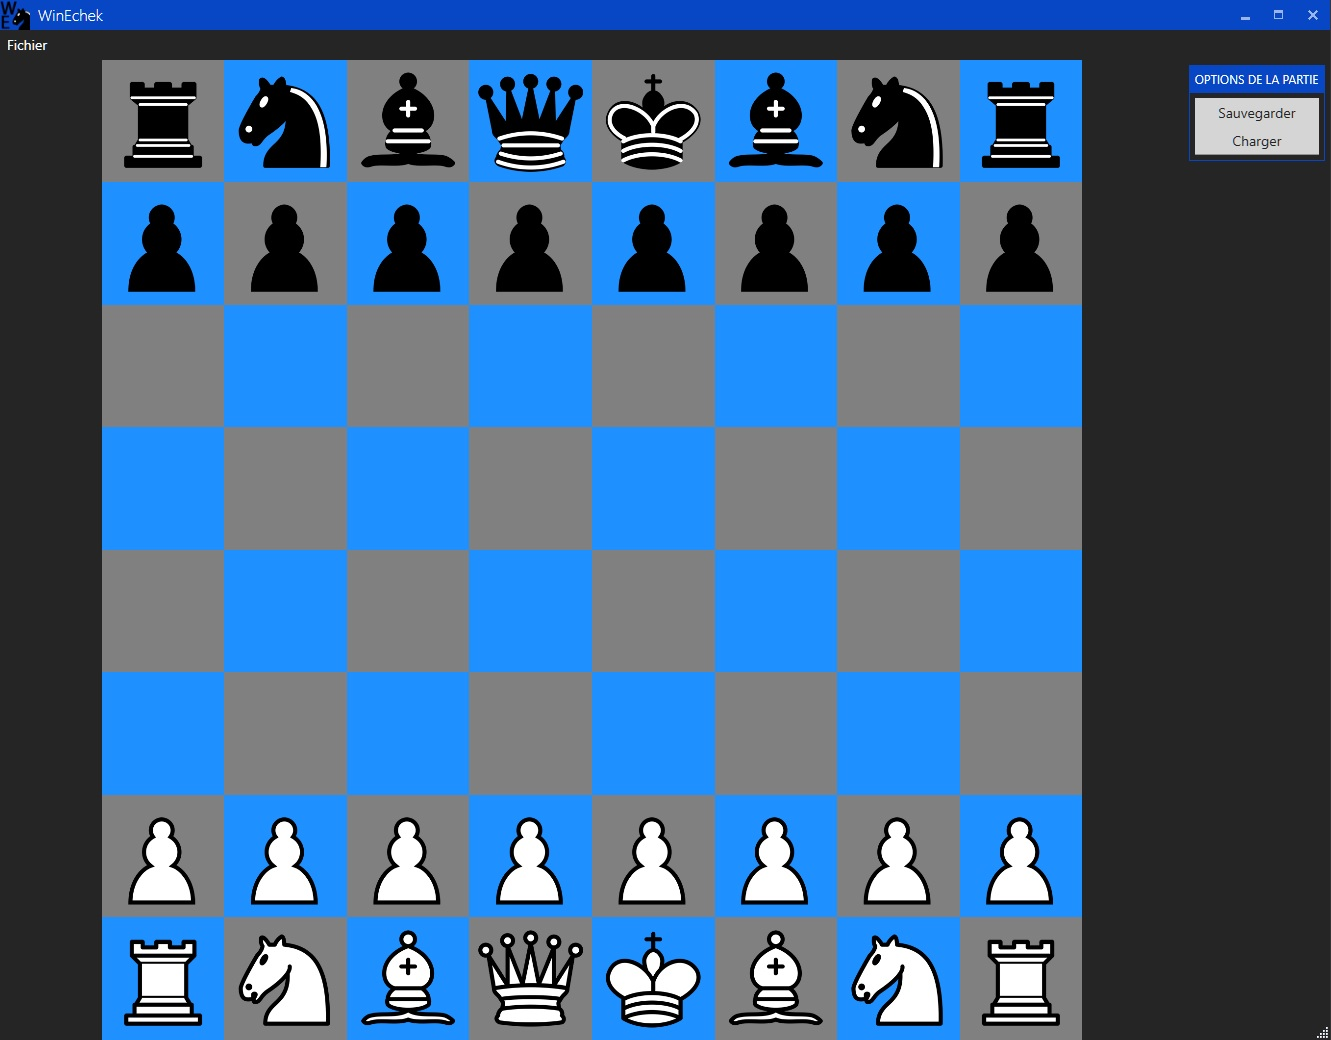
\includegraphics[width=9cm]{Images/board1.jpg}
	\end{center}
\end{frame}

\subsubsection{D�placement de pi�ces}
\begin{frame}
	\frametitle{D�placement de pi�ces}
	\begin{center}
	 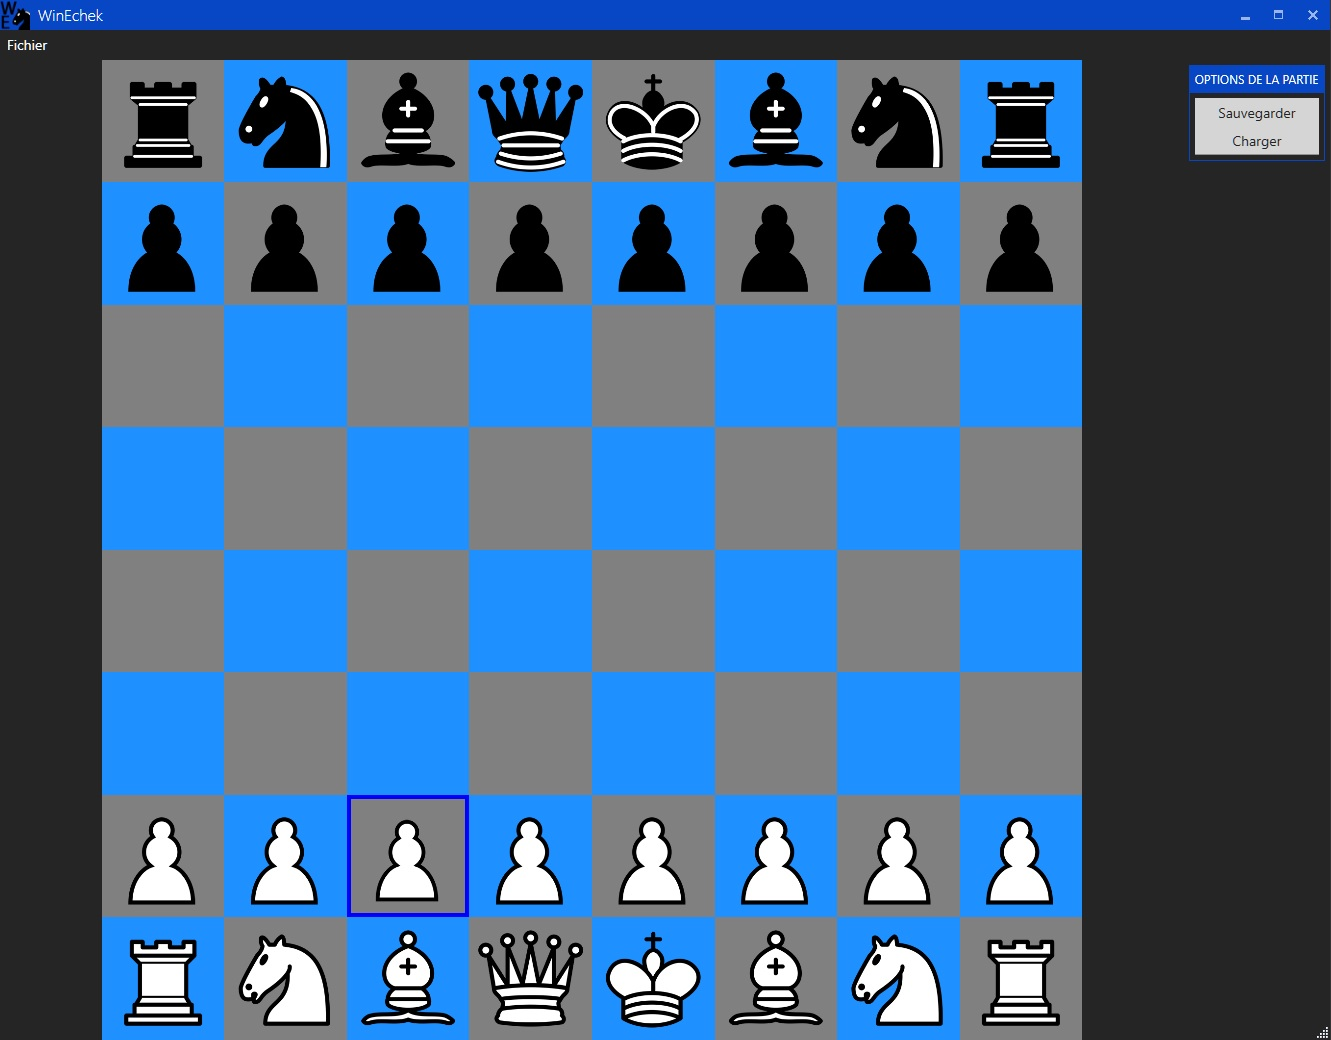
\includegraphics[width=9cm]{Images/board2.jpg}
	\end{center}
\end{frame}

\begin{frame}
	\frametitle{D�placement de pi�ces}
	\begin{center}
	 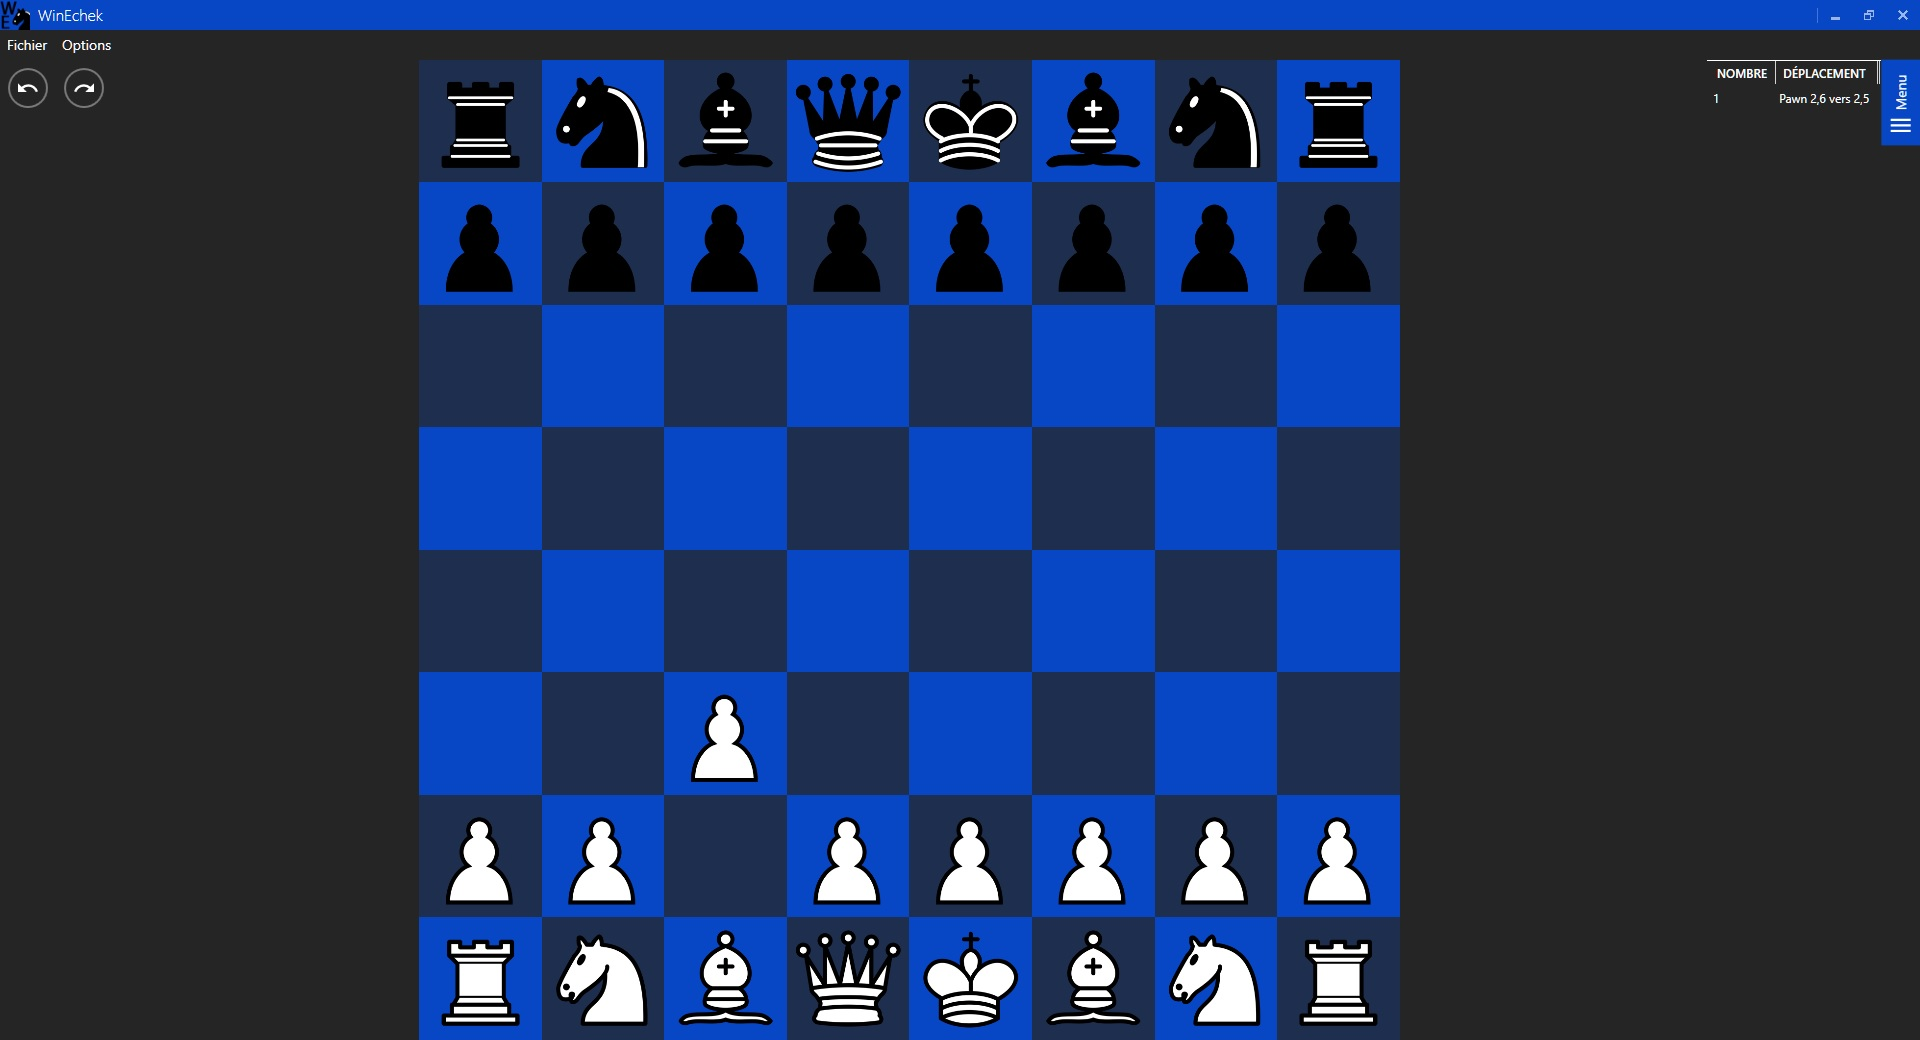
\includegraphics[width=9cm]{Images/board3.jpg}
	\end{center}
\end{frame}

\subsubsection{Options de partie}
\begin{frame}
	\frametitle{Options de partie}
	\begin{block}{Options}
		\begin{itemize}
		 \item Sauvegarder : Pour sauvegarder une partie et la reprendre plus tard
		 \item Charger : Pour charger une partie pr�c�demment sauvegarder.
		\end{itemize}
	\end{block}
	\begin{center}
	 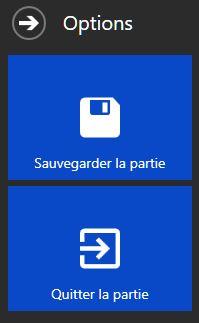
\includegraphics[width=2cm]{Images/Options.jpg}
	\end{center}
\end{frame}

\section{Prochaines fonctionnalit�s}
\subsection{Yolo}
\begin{frame}
	\frametitle{Yolo}
\end{frame}

\begin{frame}
  \frametitle{Sommaire}
  \tableofcontents
\end{frame}

\end{document}